% Chapter 7

\chapter{Resultados} % Main chapter title

\label{Chapter7} % Change X to a consecutive number; for referencing this chapter elsewhere, use \ref{ChapterX}

El objetivo de este capítulo fue el de brindar resultados para distintos escenarios de interés, con el fin de dar comparaciones analíticas con base en la variación de los parámetros de entrada del simulador.

%----------------------------------------------------------------------------------------
%	SECTION 
%----------------------------------------------------------------------------------------

\section{Escenario I} % Simulación con un solo un TTI - FER
\subsection{Descripción del escenario}
Este escenario se concentró en obtener resultados para un solo intervalo de tiempo de transmisión (TTI), con el fin de analizar el rendimiento del modelo de despliegue de UE y el modelo de canal en conjunto con NOMA y evaluar su rendimiento.
Se simuló el rendimiento de \textit{multitone} con diferentes clases de potencia para los dispositivos MTC y con diferentes tamaños de grupos ($kmax$) pero su desempeño no resultó ser importante ya que resultaba ser similar al de singletone. Por este motivo los resultados con la propuesta multitone no se reportaron. Sin embargo, en estos resultados se implementó un modo de operación híbrido donde se adoptó un modo de operación multitone solamente cuando el número de dispositivos es menor al número de grupos (48), esto con la finalidad de no desperdiciar recursos. Y singletone en los demás casos.
También es importante señalar que la relación entre dispositivos mMTC y uRLLC es de 3 a 1.
\subsection{Parámetros de entrada}
De acuerdo con los parámetros generales del modelo de sistema [véase Tabla~\ref{tab:ParametrosGral}], los criterios considerados para este escenario fueron los siguientes:
\begin{itemize} 
	\item $k_{max} \to $ 1, 2 , 3 y 4 grupos
	\item $p_{m}^{s} \to$ 23, 20, 14 dBm
\end{itemize}

\subsection{Resultados obtenidos}
En primera instancia, en el capítulo anterior se analizó el histograma de las pérdidas de canal, del Modelo CI y también del Modelo de canal que proponen en el artículo \parencite{Shahini2019} , de acuerdo con los histogramas se tiene que el valor promedio de las perdidas [dB] en el Modelo CI son de 80.35 dBs. En contrario con las pérdidas del modelo de canal del artículo en \parencite{Shahini2019}, tienen un valor promedio de 74.67 dBs. Es decir nuestro canal tiene 3.7 (5.68 dBs) veces más perdidas en comparación del canal que se implementa en \parencite{Shahini2019}, por lo que se espera que el rendimiento sea menor, esto se puede observar en la Figura~\ref{fig:NOMA_comprobacion_CI} donde se observa que en el caso de 192 usuarios el desempeño de la simulación del artículo es aproximadamente 140 usuarios, es decir 73\% de los usuarios alcanzan su tasa objetivo. Por el contrario en la evaluación de la simulación con el modelo de canal CI en NOMA se obtiene que aproximadamente 115 usuarios alcanzan su tasa objetivo, es decir, un 60\%. Hay un rendimiento del canal CI de aproximadamente 13\% del desempeño en comparación con el canal propuesto en \parencite{Shahini2019}.\newline

Cabe destacar que en \parencite{Shahini2019}, el modelo de sistema no es implementado para una banda de frecuencias en específico, las ganancias de las subportadoras son estadísticas. En el caso de este sistema como se ocupa un modelo de canal que depende de la frecuencia, se tuvo que escoger un PRB de 180 KHz, con un conjunto de subportadoras fijadas en una banda LTE, se escogió la banda de 2GHz, esto por el hecho de que LTE se implementa en bandas de microondas. \newline

\begin{figure}[th]
    \centering
    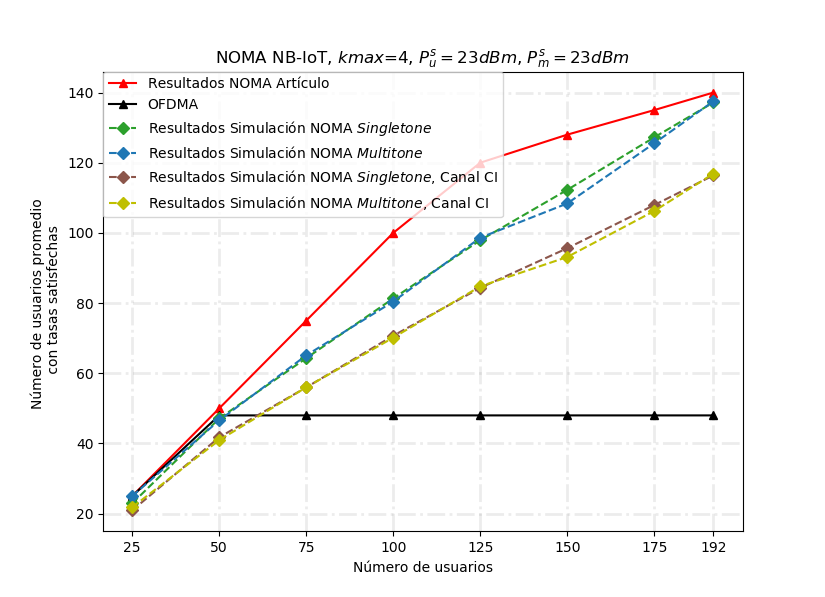
\includegraphics[scale=.7]{Figures/ResultadosNOMA/NOMA_comprobacion_CI.png}
    \decoRule
    \caption[Modelo NOMA en un TTI con modelo de canal CI]{Modelo NOMA en un TTI con modelo de canal CI}
    \label{fig:NOMA_comprobacion_CI}
\end{figure}

En la Figura~\ref{fig:NOMA_evaluacion_K_Pm_Variable_3D} se evaluó el número de usuarios que alcanzaron su tasa objetivo, se realizaron comparaciones con respecto a tres tipos de clase de potencia para los mMTC y un variable número de dispositivos por grupo (kmax).\newline

\begin{figure}[th]
    \centering
    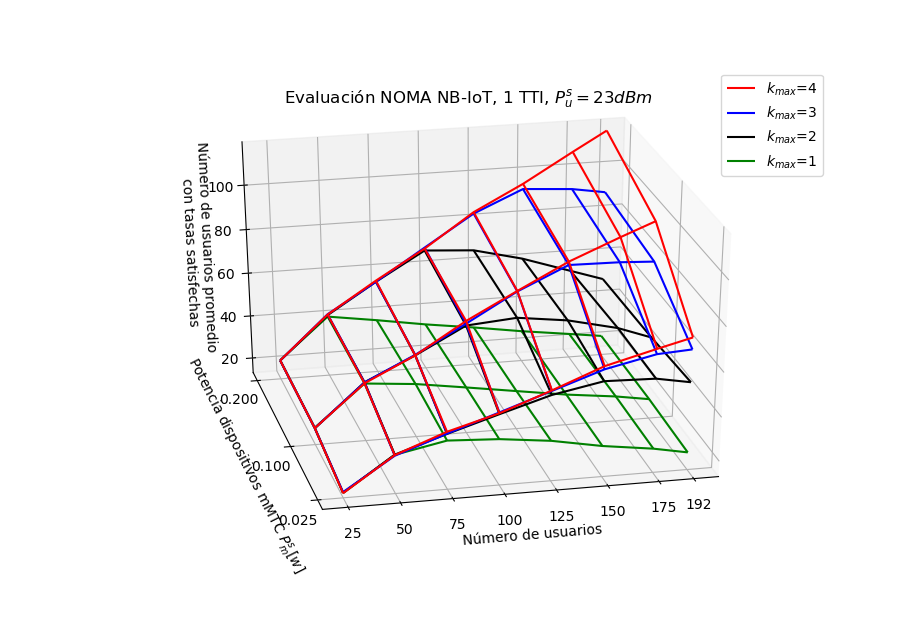
\includegraphics[scale=.7]{Figures/ResultadosNOMA/NOMA_evaluacion_K_Pm_Variable_3D.png}
    \decoRule
    \caption[Resultados generales Escenario I]{Resultados generales Escenario I}
    \label{fig:NOMA_evaluacion_K_Pm_Variable_3D}
\end{figure}

Empezando con una agrupación de 4 dispositivos, se puede observar que entre menor es la potencia de los dispositivos mMTC, el rendimiento de usuarios que alcanzan su tasa objetivo va decayendo y esto es por que al bajar su potencia los dispositivos mMTC varios de ellos comienzan a tener dificultades para alcanzar su tasa objetivo. Si se analiza el caso de 192 usuarios el desempeño con una potencia de usuarios MTC de 23dBm es de aproximadamente 115 usuarios que alcanzan su tasa objetivo, es decir, un 60\%. Y cuando la potencia de usuarios mMTC de 14dBm, 73 dispositivos alcanzan su tasa objetivo, un 38\%. Es decir el rendimiento decrece un 22\% de una potencia de 23 a 14 dBm.\newline

Con una agrupación de 3 dispositivos, vemos que el rendimiento en general decae cuando son 150 usuarios y es porque en este caso, el máximo de usuarios que pueden ser atendidos es de 144, por lo que en los casos de 175 y 192 usuarios el rendimiento va bajando esto es por la relación 3 a 1 que se propuso en los parámetros de entrada. También conforme se baja la potencia de los dispositivos mMTC, se puede ver que el rendimiento decae. Si se analiza el caso de 150 usuarios el desempeño con una potencia de usuarios MTC de 23dBm es de aproximadamente 89 usuarios que alcanzan su tasa objetivo, es decir, un 59\%. Y cuando la potencia de usuarios mMTC de 14dBm, 67 dispositivos alcanzan su tasa objetivo, un 44\%. Es decir el rendimiento decrece un 15\% de una potencia de 23 a 14 dBm.\newline

Con una agrupación de 2 dispositivos, se observa que el rendimiento en general decae cuando son 100 usuarios y es porque en este caso, el máximo de usuarios que pueden ser atendidos es de 96, por lo que en los casos mayores a 100 usuarios el rendimiento va bajando esto igualmente es por la relación 3 a 1. También, se puede ver que el rendimiento decrece cuando se baja la potencia de los dispositivos mMTC. Si se analiza el caso de 100 usuarios el desempeño con una potencia de usuarios MTC de 23dBm es de aproximadamente 53 usuarios que alcanzan su tasa objetivo, es decir, un 53\%. Y cuando la potencia de usuarios mMTC de 14dBm, 49 dispositivos alcanzan su tasa objetivo, un 49\%. Es decir el rendimiento decrece solamente 4\% de una potencia de 23 a 14 dBm.\newline

Con una agrupación de 1 dispositivo, se observa que el rendimiento en general decae cuando son 50 usuarios y es porque en este caso, el máximo de usuarios que pueden ser atendidos es de 48, por lo que en los casos mayores a 100 usuarios el rendimiento va bajando esto igualmente es por la relación 3 a 1. También conforme se baja la potencia de los dispositivos mMTC, se puede ver que el rendimiento no decae de manera significativa como lo fue en los otros casos. \newline

\break

En las siguientes figuras se evaluó la misma métrica del número de dispositivos que alcanzan su tasa objetivo pero este caso considerando cuántos de estos dispositivos son uRLLC y cuántos mMTC.\newline

\begin{figure}[th]
    \centering
    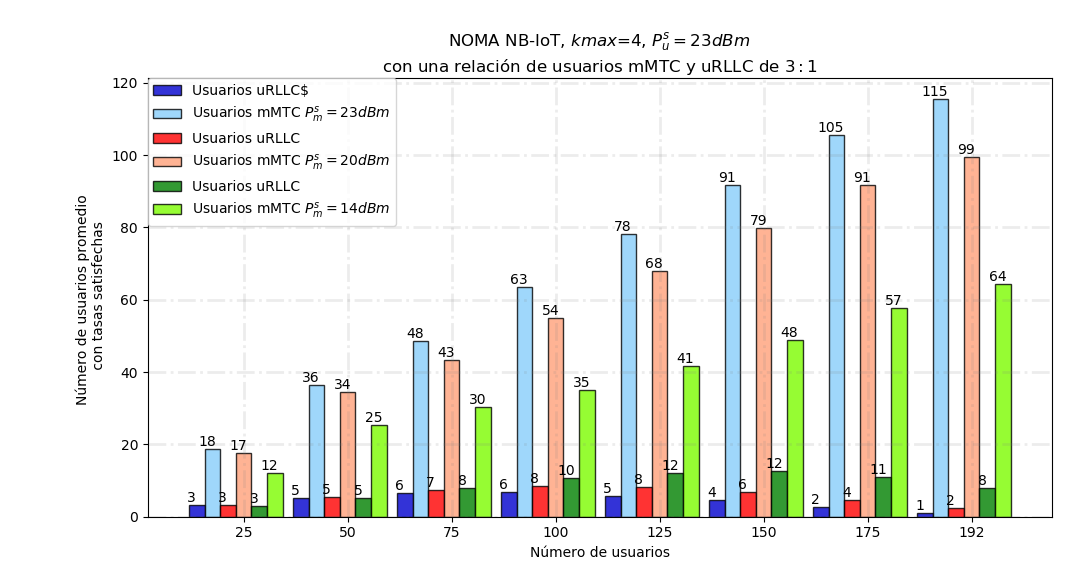
\includegraphics[scale=.65]{Figures/ResultadosNOMA/Kmax4_DiferentesPM.png}
    \decoRule
    \caption[Relación de usuarios uRLLC y mMTC que alcanzan su tasa objetivo, kmax 4]{Relación de usuarios uRLLC y mMTC que alcanzan su tasa objetivo, kmax 4}
    \label{fig:Kmax4_DiferentesPM}
\end{figure}

\begin{figure}[th]
    \centering
    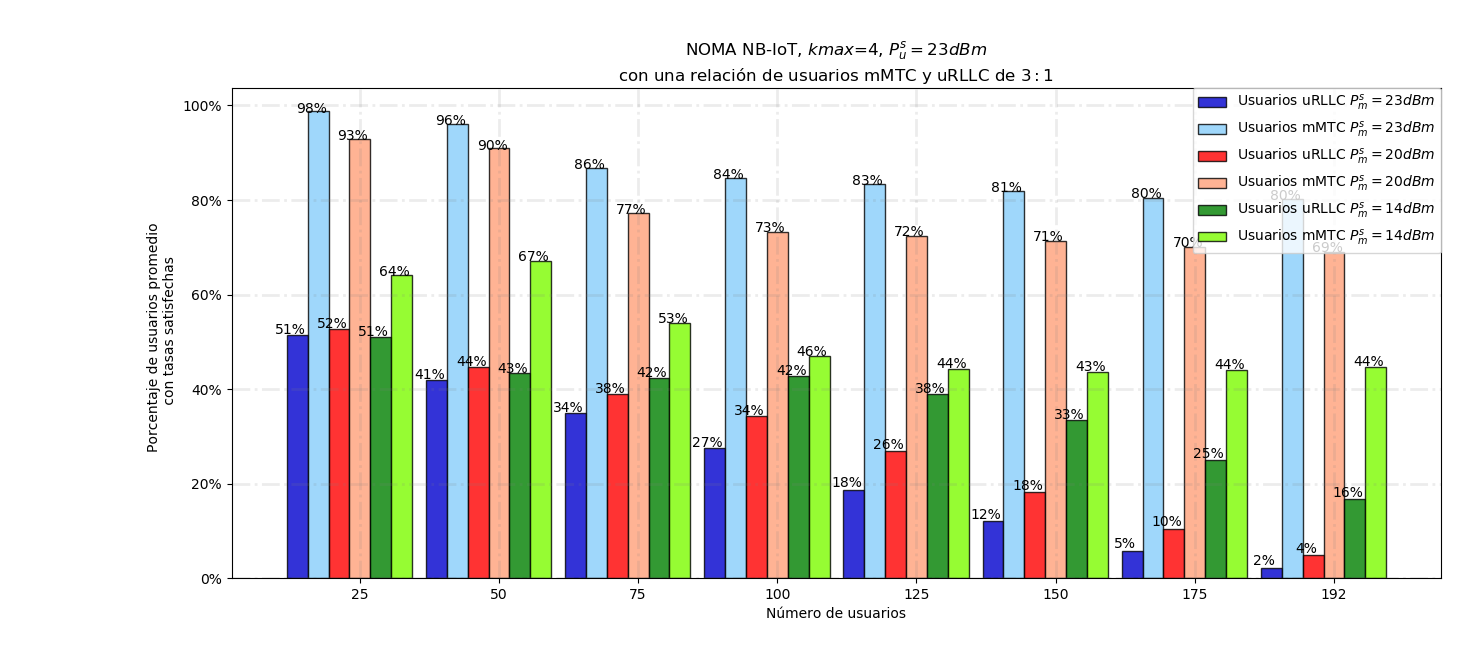
\includegraphics[scale=.65]{Figures/ResultadosNOMA/Kmax4_DiferentesPM_Porcentual.png}
    \decoRule
    \caption[Relación de usuarios uRLLC y mMTC que alcanzan su tasa objetivo $(\%)$, kmax 4]{Relación de usuarios uRLLC y mMTC que alcanzan su tasa objetivo$(\%)$, kmax 4}
    \label{fig:Kmax4_DiferentesPM_Porcentual}
\end{figure}


La Figura~\ref{fig:Kmax4_DiferentesPM} muestra la comparación del número de dispositivos mMTC y uRLLC que alcanzaron su tasa objetivo en un TTI, esto con una agrupación de 4 dispositivos (i.e. 192 dispositivos como máximo), se realizaron comparaciones con diferentes potencias de los dispositivos mMTC. Igualmente, en la Figura~\ref{fig:Kmax4_DiferentesPM_Porcentual} se representan evaluaciones acerca del número de dispositivos mMTC y uRLLC que alcanzaron su tasa objetivo, pero esta vez mostrando el porcentaje de dispositivos mMTC y uRLLC que alcanzan su tasa objetivo, de acuerdo con la relación 3 a 1 que se planteó en los parámetros de entrada.\newline

Primeramente, con una potencia de 23dBm para los dispositivos mMTC (color azul), se observa que entre mayor sea el número de dispositivos, el porcentaje de dispositivos uRLLC que alcanzan su tasa va disminuyendo, esto se puede ver más claramente en la Figura~\ref{ Kmax4_DiferentesPM_Porcentual}. Por ejemplo., cuando son 25 dispositivos el porcentaje de uRLLC y mMTC es de 51\% y 98\%, respectivamente, y cuando el número de dispositivos aumenta a 192, el porcentaje de uRLLC y mMTC es de 2\% y 80\%, respectivamente, (esto es con base en la relación 3 a 1). Como se observa la relación entre uRLLC y mMTC que alcanzan su tasa es injusta, esto debido a que al transmitir con la misma potencia todos los dispositivos, la contribución de interferencia de los dispositivos mMTC (en rangos altos) para los uRLLC, es bastante alta, impidiendo que los uRLLC no alcancen sus tasas objetivo.\newline

En los casos en donde la potencia de los dispositivos mMTC es menor a la de los uRLLC, se observa una mejor proporción entre los dispositivos. Por ejemplo, con una potencia de 14dBm para los dispositivos mMTC (color verde) el porcentaje de dispositivos uRLLC y mMTC es de 51\% y 64\%, respectivamente, y cuando el número de dispositivos aumenta a 192, el porcentaje de dispositivos uRLLC y mMTC es de 16\% y 44\%, respectivamente, (esto es con base en la relación 3 a 1). Como se observa la relación de uRLLC y mMTC que alcanzan su tasa es mas equitativa comparado con el análisis de potencia de los dispositivos mMTC con 23 dBm. \newline

\break

\begin{figure}[th]
    \centering
    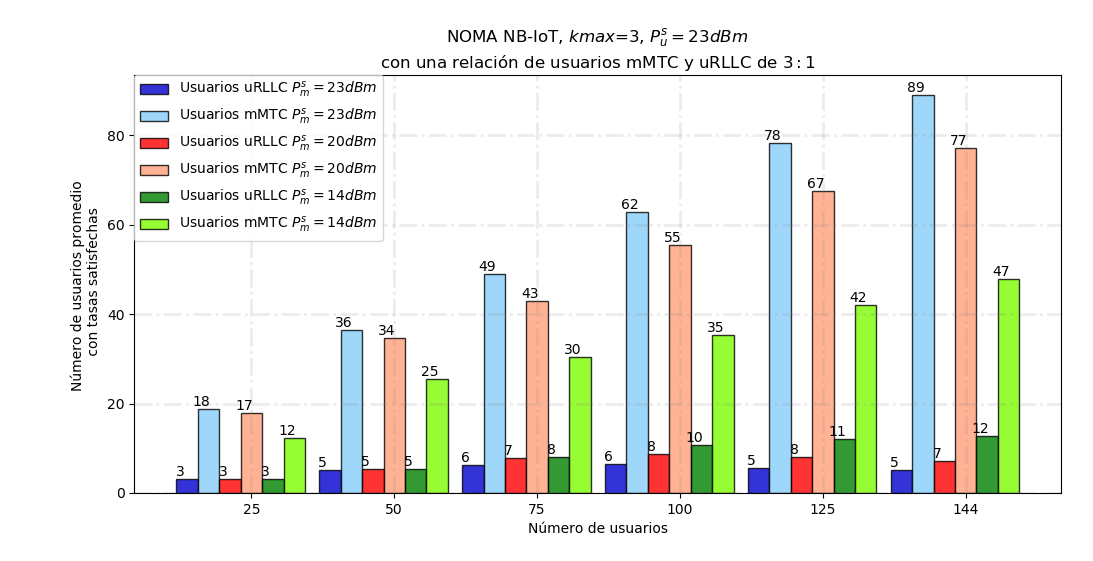
\includegraphics[scale=.65]{Figures/ResultadosNOMA/Kmax3_DiferentesPM.png}
    \decoRule
    \caption[Relación de usuarios uRLLC y mMTC que alcanzan su tasa objetivo, kmax 3]{Relación de usuarios uRLLC y mMTC que alcanzan su tasa objetivo, kmax 3}
    \label{fig:Kmax3_DiferentesPM}
\end{figure}

\begin{figure}[th]
    \centering
    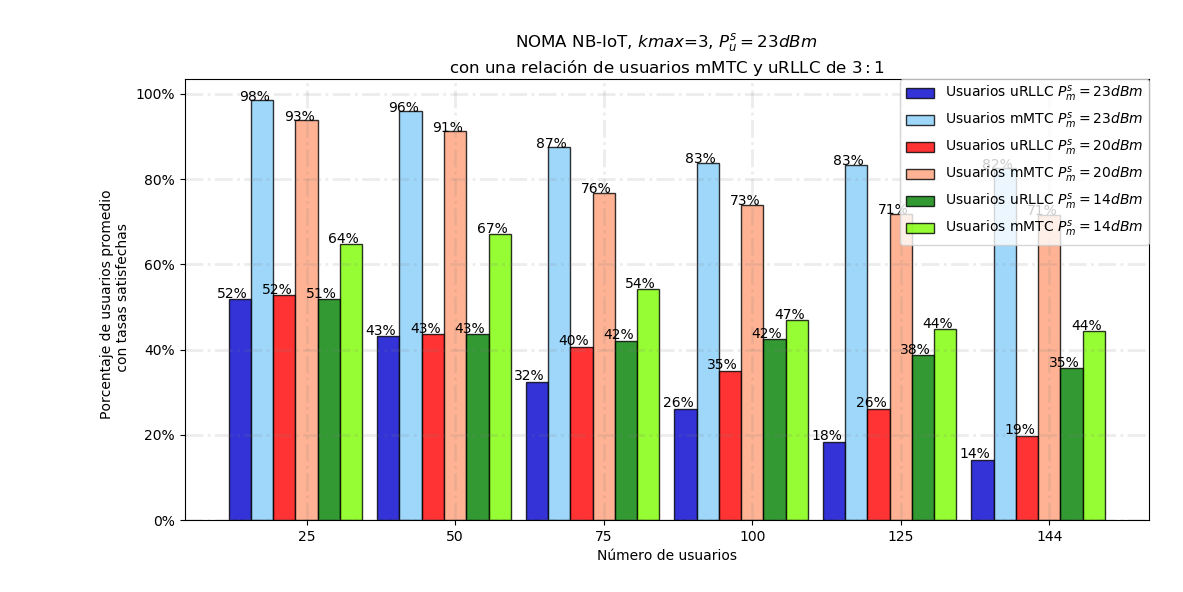
\includegraphics[scale=.65]{Figures/ResultadosNOMA/Kmax3_DiferentesPM_Porcentual.png}
    \decoRule
    \caption[Relación de usuarios uRLLC y mMTC que alcanzan su tasa objetivo $(\%)$, kmax 3]{Relación de usuarios uRLLC y mMTC que alcanzan su tasa objetivo$(\%)$, kmax 3}
    \label{fig:Kmax3_DiferentesPM_Porcentual}
\end{figure}

Las Figuras~\ref{fig:Kmax3_DiferentesPM} y ~\ref{fig:Kmax3_DiferentesPM_Porcentual} representan la relación entre el número de dispositivos mMTC y uRLLC que alcanzaron su tasa objetivo en un TTI, esto con una agrupación de 3 dispositivos (i.e. 144 dispositivos como máximo), se realizaron comparaciones con diferentes potencias de los dispositivos mMTC.\newline

Primeramente, con una potencia de 23dBm para los dispositivos mMTC (color azul), se observa que entre mayor sea el número de dispositivos, la relación de dispositivos uRLLC y mMTC que alcanzan su tasa se hace más desproporcional, esto se puede ver más claramente en la Figura~\ref{fig:Kmax3_DiferentesPM_Porcentual}. Por ejemplo, cuando son 25 dispositivos el porcentaje de dispositivos uRLLC y mMTC es de 52\% y 98\%, respectivamente, y cuando el número de dispositivos aumenta a 144, el porcentaje de dispositivos uRLLC y mMTC es de 14\% y 82\%, respectivamente, (esto es con base en la relación 3 a 1). La relación de uRLLC y mMTC que alcanzan su tasa sigue siendo injusta pero no en gran cantidad comparado con agrupaciones de 4 dispositivos, esto es porque son menos los dispositivos agrupados.\newline

En los casos en donde la potencia de los dispositivos mMTC es menor a la de los uRLLC, se observó, que se obtiene una mejor proporción entre los dispositivos. Por ejemplo, con una potencia de 14dBm para los dispositivos mMTC (color verde) el porcentaje de dispositivos uRLLC y mMTC es de 51\% y 64\%, respectivamente, y cuando el número de dispositivos aumenta a 144, el porcentaje de dispositivos uRLLC y mMTC es de 35\% y 44\%, respectivamente, (esto es con base en la relación 3 a 1). \newline

\break

\begin{figure}[th]
    \centering
    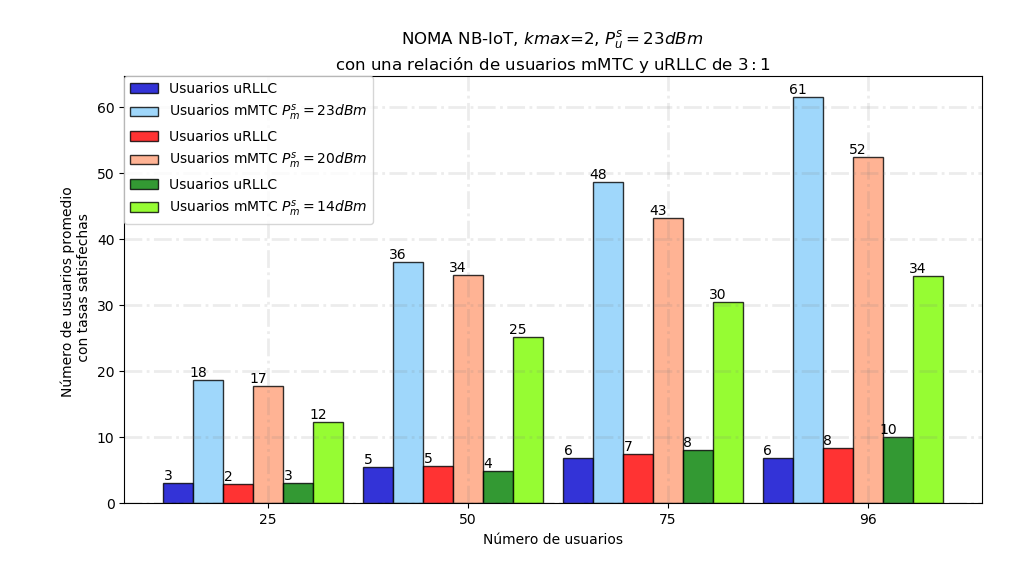
\includegraphics[scale=.6]{Figures/ResultadosNOMA/Kmax2_DiferentesPM.png}
    \decoRule
    \caption[Relación de usuarios uRLLC y mMTC que alcanzan su tasa objetivo, kmax 2]{Relación de usuarios uRLLC y mMTC que alcanzan su tasa objetivo, kmax 2}
    \label{fig:Kmax2_DiferentesPM}
\end{figure}

\begin{figure}[th]
    \centering
    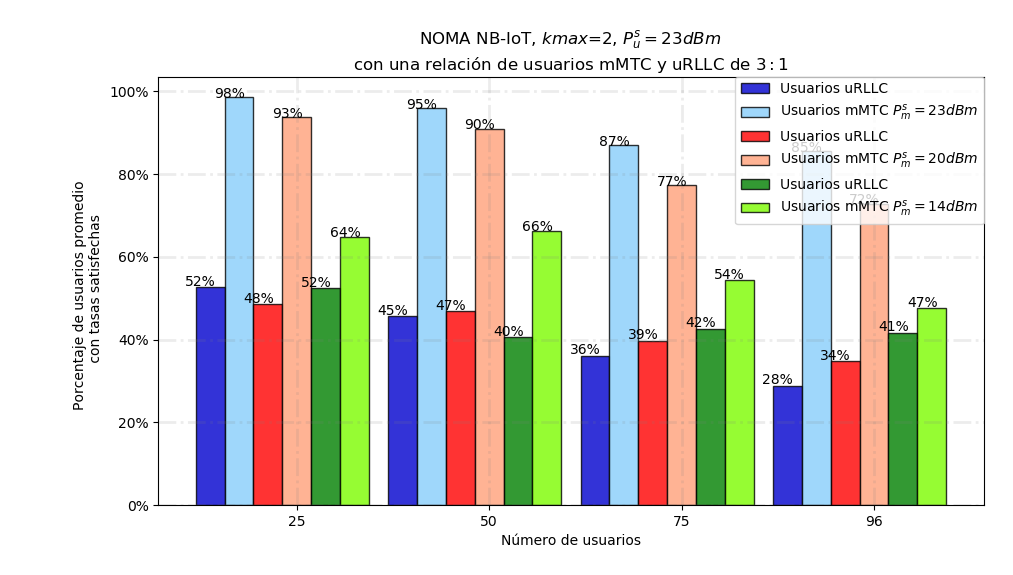
\includegraphics[scale=.6]{Figures/ResultadosNOMA/Kmax2_DiferentesPM_Porcentual.png}
    \decoRule
    \caption[Relación de usuarios uRLLC y mMTC que alcanzan su tasa objetivo $(\%)$, kmax 2]{Relación de usuarios uRLLC y mMTC que alcanzan su tasa objetivo$(\%)$, kmax 2}
    \label{fig:Kmax2_DiferentesPM_Porcentual}
\end{figure}

Las Figuras~\ref{fig:Kmax2_DiferentesPM} y ~\ref{fig:Kmax2_DiferentesPM_Porcentual} representan la relación entre el número de dispositivos mMTC y uRLLC que alcanzaron su tasa objetivo en un TTI, esto con una agrupación de 2 dispositivos (i.e. 96 dispositivos como máximo), se realizaron comparaciones con diferentes potencias de los dispositivos mMTC.\newline

Primeramente, con una potencia de 23dBm para los dispositivos mMTC (color azul), se observa que entre mayor sea el número de dispositivos, la relación de dispositivos uRLLC y mMTC que alcanzan su tasa se hace desproporcional, esto se puede ver más claramente en la Figura~\ref{fig:Kmax2_DiferentesPM_Porcentual}. Por ejemplo, cuando son 25 dispositivos, los porcentajes de dispositivos uRLLC y mMTC es de 52\% y 98\%, respectivamente, y cuando el número de dispositivos aumenta a 96 dispositivos, el porcentaje de dispositivos uRLLC y mMTC es de 28\% y 85\%, respectivamente, (esto es con base en la relación 3 a 1). \newline

En los casos en donde la potencia de los dispositivos mMTC es menor a la de los uRLLC, se observó la relación entre los dispositivos alcanzan una mejor proporción. Por ejemplo, Con una potencia de 14dBm para los dispositivos mMTC (color verde) el porcentaje de dispositivos uRLLC y mMTC es de 52\% y 64\%, respectivamente, y cuando el número de dispositivos aumenta a 144 dispositivos, el porcentaje de dispositivos uRLLC y mMTC es de 41\% y 47\%, respectivamente, (esto es con base en la relación 3 a 1). \newline


Para finalizar esta sección, se pudo observar que de la Figura~\ref{fig:NOMA_evaluacion_K_Pm_Variable_3D}, que entre menor sea la potencia de transmisión de los dispositivos mMTC, el número de dispositivos que alcanzan su tasa objetivo disminuirá, pero al hacer el análisis de las gráficas de la relación de dispositivos uRLLC y mMTC, se concluye, que aunque disminuyen los dispositivos que alcanzan su tasa, mejora equitativamente la proporción entre los dispositivos uRLLC y mMTC que logran su tasa objetivo.

\break
%----------------------------------------------------------------------------------------
%	SECTION 
%----------------------------------------------------------------------------------------

\section{Escenario II} % Simulación completa con tráfico - 

Este segundo escenario pone a prueba la capacidad que tiene el programa principal \textbf{Simulador de modelos de tráfico para nodos IoT en una red celular de 5G}, de generar resultados que permitan comparar el efecto que tiene establecer distintos parámetros de la red en el \textit{throughput} del sistema y en el porcentaje de dispositivos que cumplen su tasa deseada. \newline

\subsection{Descripción del escenario}

En este este escenario se consideraron únicamente los dispoitivos de tipo URLLC y los llamados Otros dispositivos mMTC, esto para cumplir fácilmente con la relación de 3 a 1 entre ambos tipos de dispositivos. Entonces en el programa \textbf{Generador de tráfico IoT} se generó tráfico dentro de una célula de radio igual a 200 metros. La distribución de usuarios se hizo con la opción PPP y se establecieron las intensidades de la siguiente forma: La intensidad de los dispositivos mMTC se fijo en 0.3 $dispositivos/m^2$ y la de los dispositivos URLLC se fijo en 0.1 $dispositivos/m^2$. La relación de dispositivos se eligió 3 a 1 para después fijar las tasas de nacimientos de paquetes y de alarmas idénticas en ambos tipos de servicios y garantizar que el tráfico ofrecido al sistema conserve esa relación. La tasa de nacimiento de paquetes es $\lambda_{normal} = 0.0167 paquetes/seg.$ y la de nacimiento de alarmas es $\lambda_{alarma} = 0.1 alarmas/seg.$ para ambos tipos de dispositivos. Finalmente, las características en las que se transmiten las alarmas son compartidas también entre ambos dispositivos: $velocidad_{alarma} = 500 m/s$ y para el modelo de propagación espacial se usó el modelo de ventana de coseno alzado con $d_{th}=200$ y $d_{th}=100$. \newline

De manera que virtualmente, ambos tipos los dispositivos generan tráfico a la misma tasa, pero al haber 3 veces más dispositivos mMTC, en los algoritmos NOMA se conservará en promedio esta relación.

El tráfico generado por el \textbf{Generador de tráfico IoT} correspondió a 10 segundos y la iteración seleccionada para ser evaluada por el simulador de eventos discretos contenía 2 alarmas, una para cada tipo de dispositivo, lo que es el promedio esperado, dado que $\lambda_{alarma} = 0.1 alarmas/seg.$. Se seleccionó esta iteración por ser una buena representación de los parámetros ingresados. Finalmente se inició la simulación con 48 dispositivos ya utilizando el canal, 26 dispositivos mMTC y 12 URLLC, esto para que el sistema se encontrara ya en un equilibrio de operación.

\subsection{Parámetros de entrada}

La instancia de tráfico utilizada como entrada del simulador de eventos discretos, comprendía $37541$ dispositivos mMTC y $12611$ dispositivos URLLC. El tiempo de la simulación se fijo en $10$ segundos y la potencia máxima de transmisión se fijó como $23dBm$ para los dispositivos URLLC. Finalmente se usó $d0=1m$, $PLE=2.0$ y el bloque de frecuencias que inicia en $2Ghz$. 

Se corrieron 12 rutinas en las que se variaron los valores de $k$ desde $1$ hasta $4$ y la potencia máxima de transmisión de los dispoitivos mMTC tomó valores de 23, 20 y 14 dBm.

\subsection{Resultados obtenidos}
%                                           PONER ESTO EN TABLA

Los resultados obtenidos en este escenario II se encuentran registrados en las siguientes tablas y corresponden siempre a evaluación de 12 puntos, generados apartir de las 12 combinaciones posibles de tamaño de cluster y potencia máxima de transmisión de los dispositivos mMTC. \newline

%                                           HACER ANALISIS DE GRAFICAS
\begin{figure}[th]
    \centering
    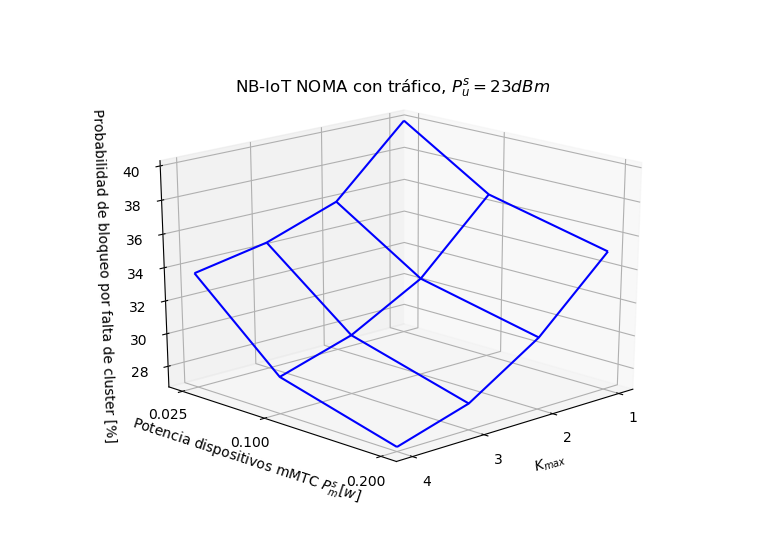
\includegraphics[scale=0.9]{Figures/ResultadosTrafico/Figure_1.png}
    \decoRule
    \caption[Probabilidad de bloque por falta de recursos]{[Probabilidad de bloque por falta de recursos}
    \label{fig:bloqueocluster}
\end{figure}

La Figura~\ref{fig:bloqueocluster}, muestra la probabilidad de bloqueo por falta de cluster. Se trata de la probabilidad que tiene cada paquete generado de ser bloqueado debido a que el dispositivo IoT no consiguió entrar a un cluster (es decir no se le asignaron recursos). Se puede notar que esta probabilidad decrece cuando se agregan más rangos a cada cluster y cuando aumenta $P_{m}^{s}$. De manera que la menor probabilidad de bloque por falta de un cluster o recursos asignados es cuando $k_{max}=4$ y $P_{m}^{s}=0.200 W$. \newline


\begin{figure}[th]
    \centering
    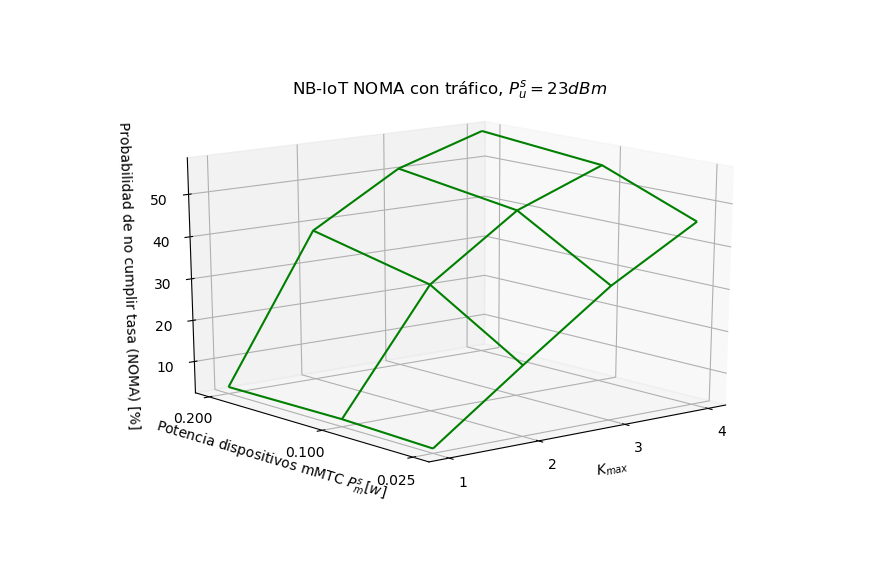
\includegraphics[scale=0.9]{Figures/ResultadosTrafico/Figure_2.png}
    \decoRule
    \caption[Probabilidad de no cumplir la tasa objetivo]{Probabilidad de no cumplir la tasa objetivo}
    \label{fig:tasa}
\end{figure}

La Figura~\ref{fig:tasa}, muestra la probabilidad que tiene cada dispositivo de no cumplir con su tasa objetivo. Esta se calcula al final de la transmisión de cada paquete, utilizando el tamaño del paquete y el tiempo que tomó transmitirlo. En la figura se puede apreciar que la menor probabilidad de que un paquete no cumpla con su tasa objetivo es para los clusters de tamaño uno, es decir cuando no se realiza NOMA. Al mismo tiempo, cuando la potencia máxima de los dispoitivos mMTC toma el valor mínimo, la probabilidad de no cumplir con la tasa objetivo parece aumentar, sin embargo se necesitarían de más corridas para concluir sobre esto. Pero pareciera que la potencia no es suficiente, cuando el tamaño de los cluster aumenta, para que todos los dispositivos mMTC cumplan con su tasa objetivo. \newline


\begin{figure}[th]
    \centering
    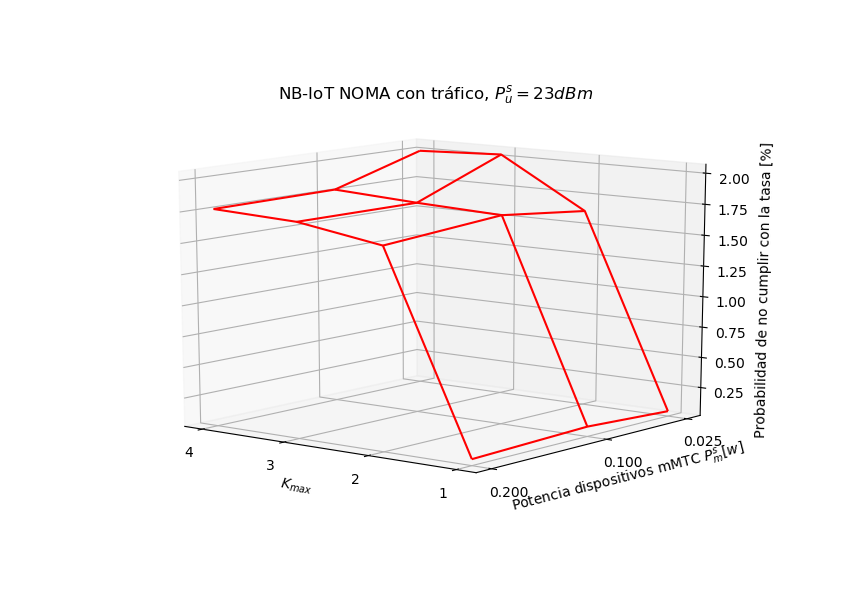
\includegraphics[scale=0.9]{Figures/ResultadosTrafico/Figure_3.png}
    \decoRule
    \caption[Probabilidad de no cumplir la tasa objetivo entre procesos NOMA]{Probabilidad de no cumplir la tasa objetivo durante un proceso NOMA}
    \label{fig:tasaNOMA}
\end{figure}

La Figura~\ref{fig:tasaNOMA}, muestra la probabilidad de que un dispositivo no consiga transmitir a su tasa objetivo al terminar un proceso NOMA y hasta el inicio del siguiente. Es importante recordar que un proceso NOMA se realiza cada que nace y cada que se termina de transmitir un paquete, de manera que muchos procesos NOMA tendrán lugar durante la transmisión completa de un sólo paquete. La tasa mostrada en la gráfica anterior podría considerarse la tasa efectiva, mientras que esta muestra la tasa en pequeños intervalos de tiempo. En la figura se puede apreciar que el orden de las probabilidades es mucho mayor que aquel en la Figura~\ref{fig:tasa}, lo que deja ver que aunque los dispositivos transmitan paquetes por debajo de su tasa objetivo durante muchos intervalos de tiempo, finalmente logran cumplir con su tasa objetivo en un porcentaje mucho mayor. Un comportamiento esperado, que se podría inferir también de esta figura es que al aumentar el tamaño de los clusters, menos dispositivos alcanzarán su tasa objetivo en estos pequeños intervalos de tiempo. Sin embargo no es tan fácil concluir esto de la tasa efectiva (La mostrada en la Figura~\ref{fig:tasa}).\newline

\begin{figure}[th]
    \centering
    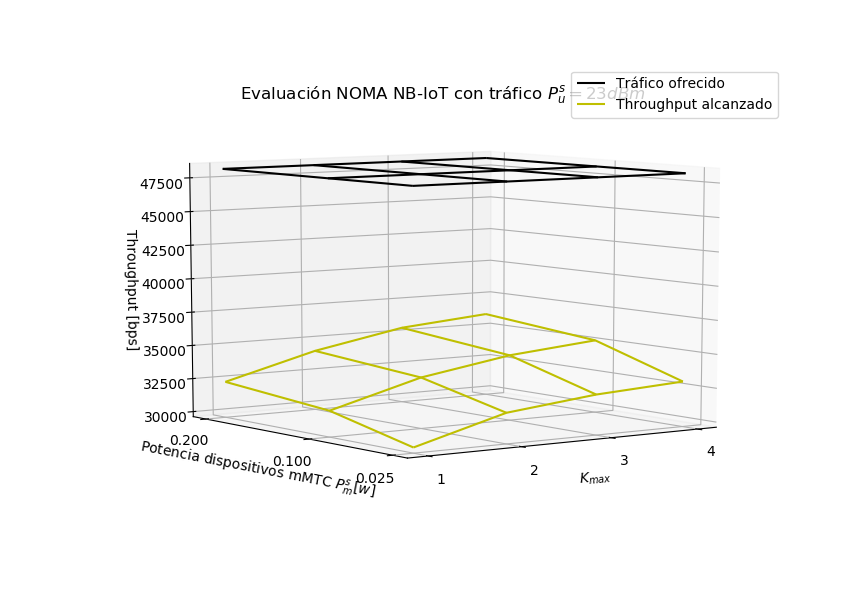
\includegraphics[scale=0.9]{Figures/ResultadosTrafico/Figure_4.png}
    \decoRule
    \caption[Throughput]{Throughput}
    \label{fig:throughput2}
\end{figure}

Finalmente, la Figura~\ref{fig:throughput2}, muestra el \textit{throughput} logrado en cada una de las 12 corridas de la simulación. Se puede ver que se logra un aumento en éste cuando se admiten más dispositivos en cada cluster y cuando aumenta la potencia de máxima de transmisión de los dispositivos mMTC.\newline 

Con ayuda de estas gráficas se puede comenzar a inferir que la mejor opción para aumentar el \textit{throughput} y reducir la probabilidad de bloqueo por falta de recursos es seleccionando $k_{max}=4$ y $P_{m}^{s}=0.200W$, a cambio claro de aumentar la probabilidad de no cumplir con las tasas objetivo de cada dispositivo. Sin embargo más corridas serían necesarias para hacer conclusiones, pero se puede apreciar que los resultados arrojados por el simulador son capaces de mostrar los efectos que tiene cambiar dos variables sobre el comportamiento del sistema.\newline